% !Mode:: "TeX:UTF-8"

\BiChapter{模型介绍}{}
在此考虑基于离散时间马氏链 $\xi = (\xi_n)_{n \ge 0}$ 建模的随机热力学系统,该模型的状态空间是 $S = \{1, \dots N\}$ 转移概率矩阵是 $P=(p_{ij})_{i,j \in S}$,其中$p_{ij}$ 表示从状态$i$到状态$j$的转移概率。该马氏链的转移图表示为 $G=(S, E)$,其中顶点集合 $S$ 是状态空间,$E$ 是转移概率有向连接边的集合。在这篇论文里,用$\langle i, j\rangle$表示状态 $i$ 到状态 $j$ 的有向边,所以有 $E = \{\langle \langle i, j\rangle \in S \times S: p_{ij}>0\}$,并且令 $M =|E|$,其中 $|E|$ 表示集合 $E$中元素的数量。本文中假设马氏链是不可约的,也就是有向图 $G$ 是连通的。因此对某个状态,图$G$不仅包含其他状态到其的边,还包括它到其自身的边,也就是自循环。

本文首先研究只有一个多于两状态的环的图 $G$ ,如图1(a) 所示,并称具有这种图结构的马氏链为单环。也就是说,如果马氏链的转移概率矩阵满足,$p_{ij}=0$ 且 $|mod(i-j, N)| \ge 2$(mod(*, N)表示模 $N$ 同余)。生化反应中的很多物理过程也都用单环马氏链建模,比如酶的构象变化,磷酸化-脱磷酸化环,染色体重塑引起的启动子激活等。本文会过多关注单环系统,很多结论也会延展到一般系统中。

\begin{figure}[h]
\centering
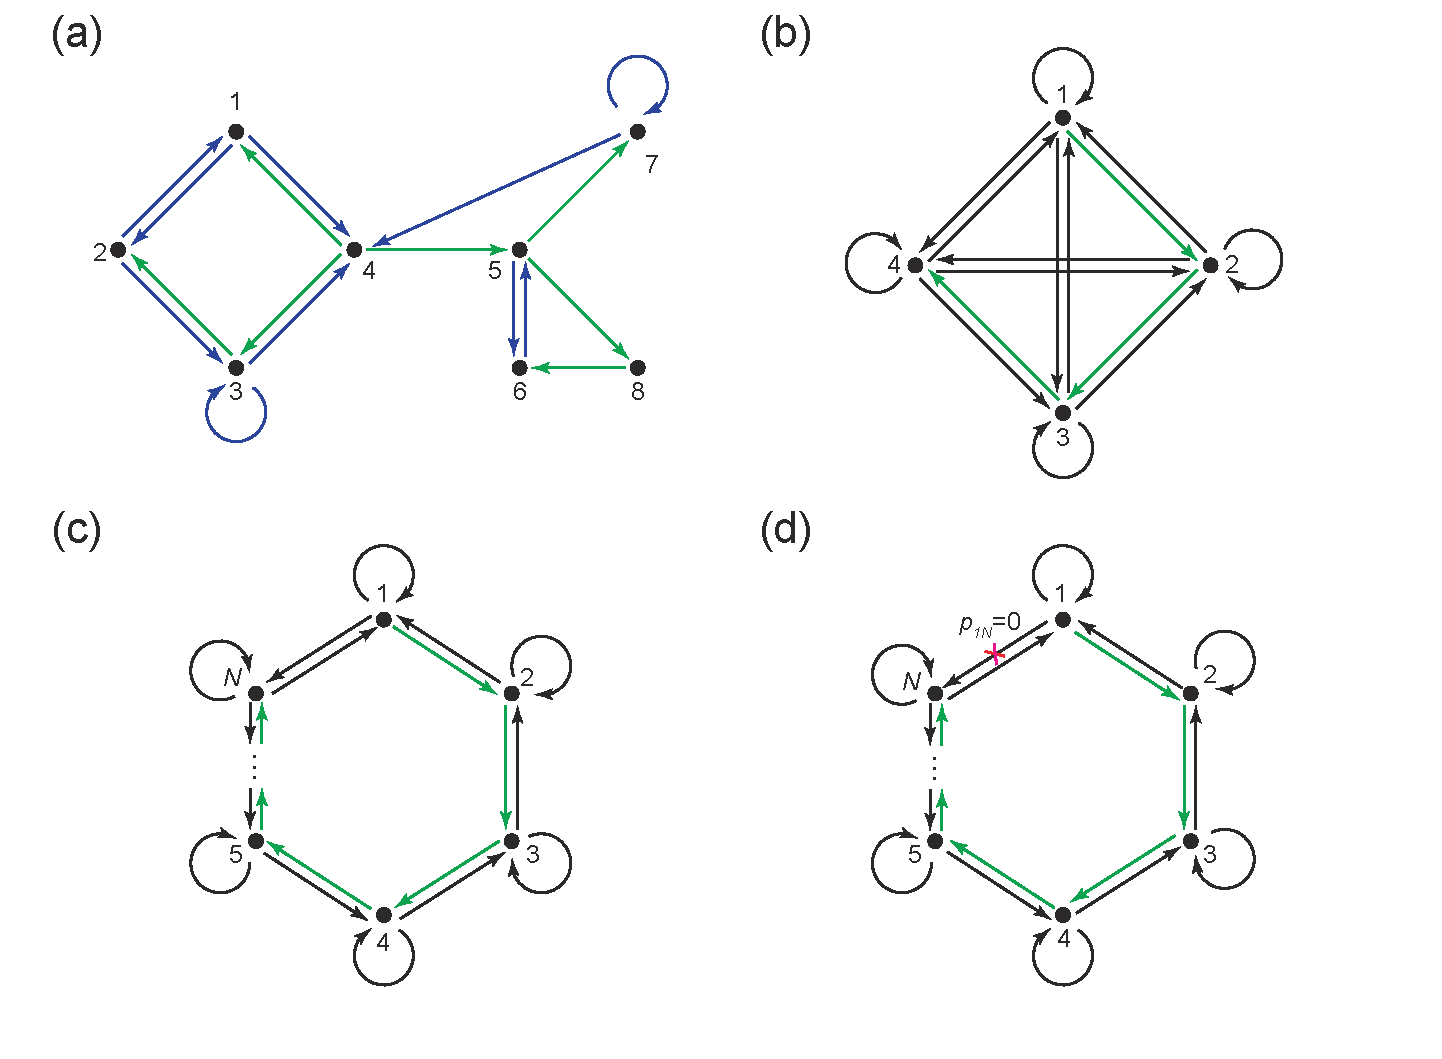
\includegraphics[scale=0.7]{chart/transitiongraph.pdf}
\caption{不同马氏链的转移图 (a) 一般马氏链的转移图, 绿色线表示生成树 $T$ ,并且蓝色线表示 $T$的弦. (b) 转移概率矩阵满足 $p_{ij}>0$ ,$\forall i, j 1\le i,j\le 4$ 的马氏链。绿色线表示生成树 $T=1\to 2\to 3\to 4$. (c) $N$状态单环马氏链。绿线表示生成树 $T=1\to 2\to \cdots\to N$. (d) 转移概率矩阵有$p_{1N}=0$的单环马氏链,绿色线表示生成树 $T=1\to 2\to \cdots\to N$.}\label{figure:transitiongraph}
\end{figure}

\BiSection{环擦除定义下的环流}{}
本文研究马氏链中两种类型的环流,该章节回顾环擦除定义下的环流。马氏链中的回路是用路径定义的,比如路径 $i_1 \to i_2 \to\cdots\to i_s \to i_1$($i_1, i_2 , \cdots, i_s$是顶点集合$S$中不同点)的环流为 $p_{i_1i_2}p_{i_2i_3}\cdots p_{i_si_1}>0$。令 $j_1 \to j_2 \to\cdots\to j_r \to j_1$ 为另一个环,若上述两个环满足存在一个整数 $k$ 使得
\begin{equation*}
    j_1 = i_{k+1},j_2 = i_{k+2},\cdots,j_n = i_{k+s},
\end{equation*}
且 $r=s$ 则称两个回路是等价的,其中指标 $k+1,k+2,\cdots,k+s$ 被视为模 $n$ 同余的。环流 $i_1 \to i_2 \to\cdots\to i_s \to i_1$ 在上述等价关系下所属的等价类被表示为 $(i_1,i_2,\cdots,i_s)$。例如,$(1,2,3)$, $(2,3,1)$ 和 $(3,1,2)$表示相同的环。环$(i_1,i_2,\cdots,i_s)$ 的反环被定义为 $(i_1,i_s,\cdots,i_2)$。通常称马氏链中所用环的集合为环空间 $\mathcal{C}$。

马氏链的一条轨迹会形成各种换。直观看,如果我们抛弃马氏链 $\xi$ 中环,并且在该过程中,始终关注轨迹中剩余状态形成的轨道,那么称剩余的轨迹为导出链 $\tilde{\xi} = (\tilde{\xi}_n)_{n\geq 0}$ 。例如,如果马氏链 $\xi$ 的轨迹为 $\{1,2,3,3,2,3,4,1,4,\cdots\}$,那么相应的导出链 $\tilde{\xi}$ 的轨迹和环形成为表1所示 
\begin{table}[htb!]
    \renewcommand\arraystretch{1.3}\centering
    \begin{tabular}{cccccccccc} \hline\hline
    $n$             & 0 & 1 & 2 & 3   & 4     & 5 & 6 & 7         & 8 \\ \hline
    $\xi_n$          & 1 & 2 & 3 & 3   & 2     & 3 & 4 & 1         & 4 \\ \hline
    $\tilde{\xi}_n$ & {[}1{]} & {[}1,2{]} & {[}1,2,3{]} & {[}1,2,3{]} & {[}1,2{]} & {[}1,2,3{]} & {[}1,2,3,4{]} & {[}1{]} & {[}1,4{]} \\ \hline
    \text{环} &   &   &   & (3) & (2,3) &   &   & (1,2,3,4) &   \\ \hline\hline
    \end{tabular}
    \caption{导出链和形成的环}\label{trajectory}
\end{table}

特别地,导出链的状态用 $S$ 的中状态组成的有限序列表示,即 $[i_1,i_2,\cdots,i_s]$。假设 $\tilde{\xi}_{n-1}=[i_1,i_2,\cdots,i_s]$ 且 $\xi_n = i_{s+1}$。若 $i_{s+1}$ 不同于 $i_1,i_2,\cdots,i_s$,那么$\tilde{\xi}_n$ 被定义为 $\tilde{\xi}_n = [i_1,i_2,\cdots,i_s,i_{s+1}]$。其次,若$i_{n+1}=i_r$,那么 $\tilde{\xi}_n$ 被定义为 $\tilde{\xi}_n = [i_1,i_2,\cdots,i_r]$。对于这种情况,称马氏链在时间 $n$ 形成环 $(i_r,i_{r+1},\cdots,i_s)$。令 $N^c_n$ 为环 $c$ 在时间 $n$ 时形成的次数。那么在时间 $n$ 时,环 $c$ 的经验环流可以被定义为:
\begin{equation*}
    J_n^c = \frac{1}{n}N^c_n,
\end{equation*}
并且在时间 $n$ 时,经验净环流可以定义为:
\begin{equation*}
    \tilde{J}^c_n = J^c_n-J^{c-}_n.
\end{equation*}
用更直观的表述,$J^c_n$ 表示环$c$ 平均每个单位时间形成的数量,$\tilde{J}^c$ 表示环$c$ 平均每个单位时间形成的净数量。
若令 $n\rightarrow\infty$,则有经验环流 $J^c_n$ 和 经验净环流 $\tilde{J}^c$ 分别以概率为 1 趋近于 $J^c$ 和 $\tilde{J}^c$。
极限 $J^c$ 和 $\tilde{J}^c$ 分别被视为环 $c$ 的环流和净环流。关于$J^c_n$ 和 $\tilde{J}^c$ 更为细致的描述,可以参考文献 [1]。著名的环流分解定理可以用上述定义表示为:
\begin{equation}\label{decomposition}
    \pi_ip_{ij} = \sum_{c\ni\langle i,j\rangle}J^c,
\end{equation}
其中 $c \ni \langle i, j\rangle$ 表示环 $c$ 中有边 $\langle i, j\rangle$。

\BiSection{生成树定义下的环流}{}
环的环流可以用生成树的方式定义。令 $T$ 为 $G$ 的一个有向子图,也就是说 $T$ 的所有边也是 $G$ 的边,再令$\hat{T}$ 表示 $\bar{T}$ 表示与 $T$ 有关的无向图。
满足下列三个条件的 $T$ 被称为图 $G$ 的生成树:
\begin{itemize}
    \item $T$ 是 $G$ 的覆盖子图,也就是说 $T$ 包含 $G$ 的所有顶点。
    \item $\bar{T}$ 是连通的。
    \item $\bar{T}$ 没有回路,其中无向图的回路是顶点到自身的无向路径。
\end{itemize}

易知生成树 $T$ 包含 $G$ 的所有顶点,并且 $|T| = N -1$。接下来,会通过 $T$ 表示生成树和它的边集合。图的生成树并不唯一,一个图可以有很多完全不同的生成树。

若有向边 $l \notin T$,则被称为 $T$ 的弦。(图1 a)。因为 $|T|= N-1$,生成树 $T$ 有 $M-N+1$ 个弦,也就是说明图 $G$ 中有 $M-N+1$ 条边不会在 $T$ 中出现。同时 $\bar{T}$ 是连通的,并且没有环的,如果添加一根弦 $l$ 到 $T$,则导出的子图 $\overline{T \cup \{l\}}$ 会恰巧有一个回路,表示其为 $C_l$。记 $c_l$ 是从 回路 $C_l$ 中获得的环,并且和 $l$ 保持同样的指向。由弦生成的环的集合 $\mathcal{L} = \{c_l: l\in E\setminus T\}$ 被称为基本集。很明显,弦和基本集之间没有一一对应的关系,可以用 $c_l$ 形成的次数定义通过弦 $l$ 的次数。那么经验时间 $n$ 时刻,$c_l$ 的经验环流可以被定义为:
\begin{equation*}
    Q^{c_l}_n = \frac{1}{n}\sum_{i=1}^n1_{\{\langle\xi_{i-1},\xi_i\rangle=l\}}.
\end{equation*}
$Q^{c_l}_n$ 表示单位时间通过弦 $l$ 的次数。生成树方式和环擦除方式有很大的不同,环擦除可以很便捷的定义环流,生成树只能定义基本集的环流。

类似的,也可以用生成树定义净环流。最终,假设转移概率满足 $p_{ij}>0$,当且仅当 $p_{ji}>0$,这个条件可以保障熵增量是有限的。【1】考虑 $l
$,在时间步 $n$,$c_l$的净环流定义为:
\begin{equation*}
    \tilde{Q}^{c_l}_n=Q^{c_l}_n-Q^{c_l-}_n.
\end{equation*}
如果 $c_l$ 中只有一个或两个状态,那么易知 $c_l = c_{l^-}$,因此 $\tilde{Q}_n^{c_l}=0$。对于弦 $l=\langle i,j \rangle$,如果 $c_l$中有三个以上的状态,那么 $l^-$ 也是一个弦,并且 $c_{l^-}$ 是由弦 $l^-$ 生成的环。在文献 [3-6],净环流的定义只是考虑有三个及以上状态的的环,本文参考文献【2】中的定义,使得净环流的定义也可以包含只有一个或两个状态的环。

若 $n \to \infty$, 则经验环流 $Q_n^{c_l}$ 和经验净环流 $\tilde{Q}_n^{c_l}$ 将会分别以概率为 $1$ 趋于 $Q^{c_l}$ 和 $\tilde{Q}^{c_l}$。极限 $Q^{c_l}$ 和 $\tilde{Q}^{c_l}$ 分别被当做环 $c$ 的环流与净环流。根据马氏链的遍历性,有 $Q^{c_l} = \pi_i p_{ij}$。

\BiSection{两种类型环流的比较}{}
下面将简述两种类型环流的差异。为叙述简便,由环擦除方式定义的环流称为 $LE$ 环流,由生成树方式定义的环流称为 $ST$ 环流。$LE$ 环流是对环空间 $\mathcal{C}$ 中所有环定义的,然而 $ST$ 环流仅是针对基本集 $\mathcal{L}$ 定义的。因此,对于马氏链的环动态性,$LE$ 环流相较于 $ST$ 环流给出了更完整的描述。而且,由于生成树不具有唯一性,不同的生成树选择会对应不同的 $ST$ 环流。对比之下,$LE$ 环流并不依赖生成树的选择。

经过上述的比对,自然会问到基本集 $\mathcal{L}$ 和环空间 $\mathcal{C}$ 的差距会有多大。因为每根弦对应集合 $\mathcal{L}$ 唯一一个元素,即 $|\mathcal{L}| = |E\setminus T| = M-N+1$,所以很难对 $|\mathcal{C}|$ 给出一般性的表述。下面将主要考虑几个重要的特例。首先考虑转移图是全连接的马氏链(图1b),也就是 $p_{ij}>0, \forall i,j \in S$。